\documentclass[11pt,letterpaper]{article}
\usepackage[margin=0.75in]{geometry}
\usepackage[T1]{fontenc}
\usepackage{lmodern}
\usepackage{amsmath,amssymb}
\usepackage{graphicx}
\usepackage{booktabs}
\usepackage[font=small,labelfont=bf,skip=3pt]{caption}
\usepackage{float}
\usepackage{xcolor}
\definecolor{darkred}{HTML}{8B0000}
\newcommand{\new}[1]{\textcolor{darkred}{#1}}
\usepackage[hidelinks]{hyperref}
\graphicspath{{figures/}{./}}
\setlength{\parskip}{0.3em}
\setlength{\intextsep}{6pt}
\setlength{\floatsep}{6pt}
\setlength{\textfloatsep}{6pt}
\setlength{\parindent}{0pt}
\renewcommand{\thetable}{S\arabic{table}}
\renewcommand{\thefigure}{S\arabic{figure}}

\title{\Large\bfseries Supplementary Information for\\ SilentMethyl: a multimodal framework for CpG methylation prediction and local variant-effect inference}
\author{Samuel Zhang, Shaojun Pei, and Gil Alterovitz}
\date{\vspace{-2.5em}}

\begin{document}
\maketitle

All results use the primary breast-epithelium models and the held-out test chromosomes 8 and 9 unless stated otherwise. Intervals are 95\% confidence intervals. Source data for every figure panel are in \texttt{figures/source\_data/} of the code repository.

\section*{Supplementary Results}
\label{sec:supplementary_results}
\subsection*{Prediction disagreement and motif analyses help assess model limitations}
Differences between forward and reverse-complement predictions were associated with single probe prediction error, with a rank correlation near 0.50 between them. In addition, distance to $\beta = 0.5$ appeared useful in identifying inaccurate probe predictions, possibly because methylation $\beta$ is bimodally distributed and restricted to the range of $[0, 1]$. However, its usefulness weakened when error was measured on the unbounded $M$ scale (Supplementary Figs.~\ref{fig:uncertainty} and~S3a). 

These results show why model error should be checked on more than one numerical scale. Forward/reverse-complement disagreement can help rank how unreliable baseline CpG predictions are, but does not provide a validated prediction interval or establish the error in a variant-effect prediction. The disagreement remains helpful for checking model consistency, although consistency alone does not establish biological accuracy.

We also examined if DNA motif changes could help explain predicted differences in methylation. Among 831 JASPAR motifs, the strongest relationships involved similar ETS motifs sharing the GGAA core. Weaker motif scores were linked to increases in predicted methylation. These relationships were strongest in the $k$-mer ridge model. However, overall motif disruption showed little to no correlation with predicted effects ($\rho=-0.0103$, $-0.0220$ to 0.0019). Additionally, the model performed similarly in separating significant mQTLs from controls among variants with strong motif disruption and matched variants with weak motif disruption. AUROC was 0.595 (0.574--0.616) on strong versus 0.595 (0.574--0.618) on weak (Supplementary Figs.~\ref{fig:motifs} and~S3b). These results suggest some model sensitivity to sequence composition and motif patterns, but do not establish that the model learned transcription factor binding.

\vspace{-0.6em}\section*{Supplementary tables}

\begin{table}[H]
\centering
\caption{\textbf{Baseline methylation prediction on 26,570 held-out CpGs.} Values are mean $\pm$ standard deviation across seeds 42--44. The two ridge models are single fits. CpGenie and DeepCpG (DNA module only) were retrained on the same splits.}
\label{tab:s1}
\small
\begin{tabular}{lccc}
\toprule
Model & $\beta$ MAE & $M$ MAE & ROC-AUC\\
\midrule
Composition ridge & 0.1954 & 1.9600 & 0.8748\\
$k$-mer ridge & 0.1565 & 1.6866 & 0.9190\\
CpGenie & $0.1281\pm0.0013$ & $1.3858\pm0.0103$ & $0.9406\pm0.0006$\\
DeepCpG & $0.1253\pm0.0005$ & $1.3412\pm0.0112$ & $0.9437\pm0.0011$\\
Context & $0.1022\pm0.00003$ & $1.1763\pm0.0005$ & $0.9658\pm0.00001$\\
Sequence & $0.1099\pm0.0008$ & $1.1941\pm0.0070$ & $0.9569\pm0.0007$\\
Fusion & $0.0914\pm0.0037$ & $1.0341\pm0.0289$ & $0.9744\pm0.0025$\\
\bottomrule
\end{tabular}
\end{table}

\begin{table}[H]
\centering
\caption{\textbf{Allele-specific methylation (ASM) results for each model.} All tests use seed 42. Intervals use 2,000 resamples of 1-Mb genomic blocks. For Do--Tycko signed tests, predicted $\Delta\widehat M$ was averaged across the scored CpGs in each SNP's DMR. Rosenski--Dor--Kaplan controls are loci with bimodal methylation but no ASM; Do--Tycko controls are loci outside DMRs. Both control sets were matched to the ASM loci by variant--CpG distance.}
\label{tab:s2}
\small
\begin{tabular}{llccc}
\toprule
\multicolumn{5}{l}{\textit{Do--Tycko signed agreement (722 SNPs, 328 with positive measured effects, 179 blocks)}}\\
Model & & Direction agreement & Signed Spearman $\rho$ & Directional AUROC\\
\midrule
Fusion & & 0.590 (0.550--0.630) & 0.241 (0.180--0.299) & 0.628 (0.584--0.669)\\
Sequence & & 0.591 (0.554--0.629) & 0.250 (0.193--0.306) & 0.631 (0.588--0.671)\\
\midrule
\multicolumn{5}{l}{\textit{Separating ASM from controls (AUROC)}}\\
Cohort & Pairs (blocks) & Fusion & Sequence & Distance only\\
\midrule
Rosenski--Dor--Kaplan & 6,910 (242) & 0.562 (0.533--0.593) & 0.574 (0.545--0.601) & 0.502 (0.478--0.524)\\
Do--Tycko & 10,746 (179) & 0.542 (0.508--0.580) & 0.543 (0.502--0.585) & 0.503 (0.480--0.531)\\
\bottomrule
\end{tabular}
\end{table}

\begin{table}[H]
\centering
\caption{\textbf{Prediction changes after shuffling context or replacing it with feature medians.} Seed-42 fusion predictions on 76,893 held-out eGTEx breast pairs, compared with predictions using the original context. Normalized change is the mean absolute change divided by the standard deviation of the original predictions. Levels are baseline $\widehat M$; effects are $\Delta\widehat M$.}
\label{tab:s3}
\small
\begin{tabular}{llcccc}
\toprule
Context & Prediction & Normalized change & Spearman $\rho$ & Pearson $r$ & Sign agreement\\
\midrule
Shuffled & Levels & 0.5260 & 0.6180 & 0.6324 & 0.7522\\
Shuffled & Effects & 0.2266 & 0.7755 & 0.7528 & 0.8440\\
Median & Levels & 0.3530 & 0.9430 & 0.9525 & 0.9428\\
Median & Effects & 0.1860 & 0.8047 & 0.8624 & 0.8355\\
\bottomrule
\end{tabular}
\end{table}

\vspace{-0.6em}\section*{Supplementary figures}

\begin{figure}[H]
\centering
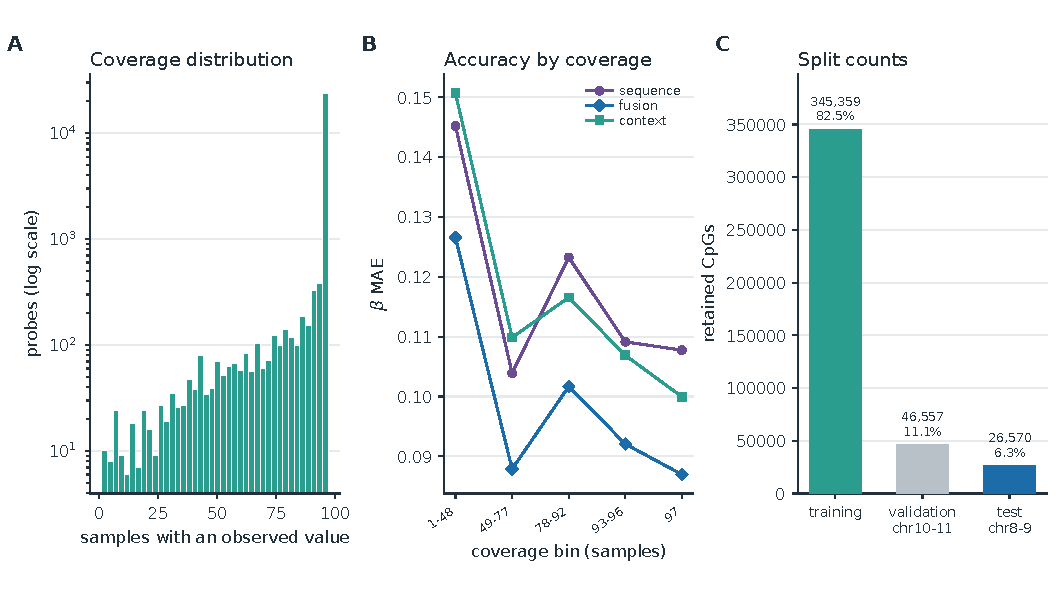
\includegraphics[width=\textwidth]{figS1_target_split_qc.pdf}
\caption{\textbf{Target coverage and data splits.}
\textbf{a}, Number of samples with a measured value at each of the 26,570 held-out CpGs.
\textbf{b}, $\beta$ MAE by coverage group for the three SilentMethyl models.
\textbf{c}, CpGs in each chromosome split. Splits are by chromosome, not by patient, so all 97 samples contribute to every split.}
\label{fig:s1}
\end{figure}

\begin{figure}[H]
\centering
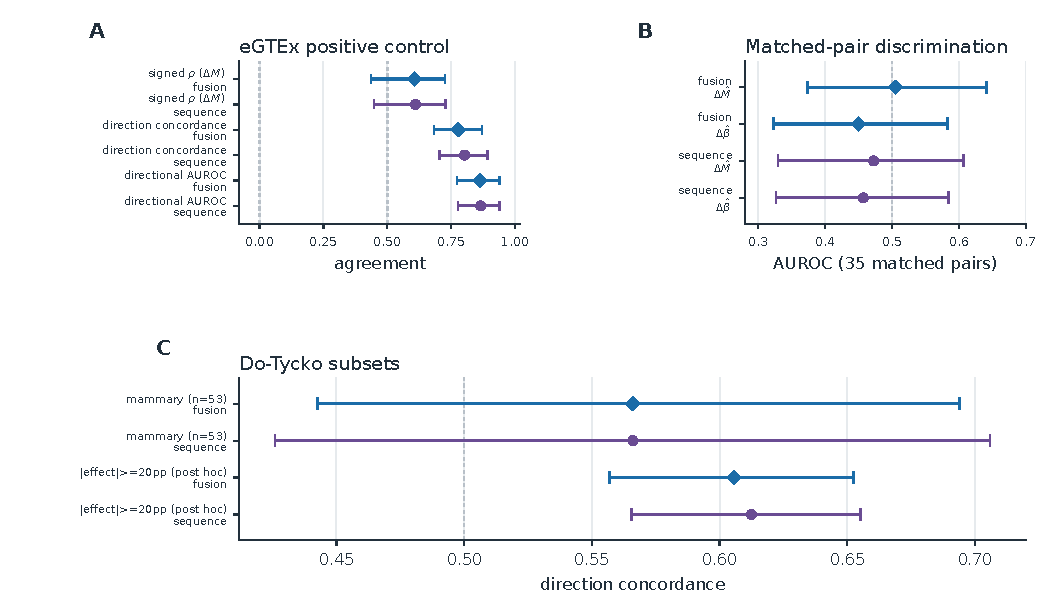
\includegraphics[width=\textwidth]{figS2_external_controls.pdf}
\caption{\textbf{Additional external controls.}
\textbf{a}, eGTEx breast lead-mQTL positive control (81 associations from 70 variants). Intervals use 10,000 resamples of variants; dashed lines mark chance (0 for correlation, 0.5 for the rates).
\textbf{b}, AUROC for 35 matched pairs of significant and high-$q$ lead variants. Intervals use 5,000 resamples of matched pairs.
\textbf{c}, Do--Tycko direction agreement in the 53 mammary SNPs and in the 578 SNPs with measured effects of at least 20 percentage points. The second subset was chosen after the main analysis. Intervals use 2,000 resamples of 1-Mb blocks.}
\label{fig:s2}
\end{figure}

\begin{figure}[H]
\centering
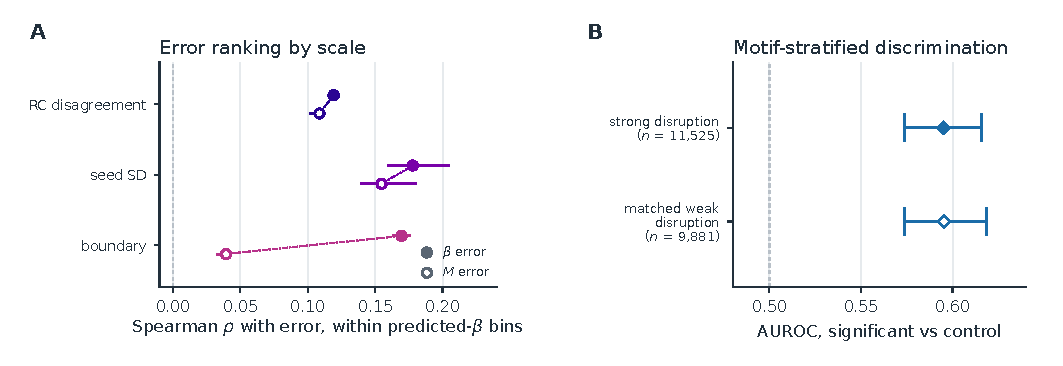
\includegraphics[width=\textwidth]{figS3_uncertainty_motif_controls.pdf}
\caption{\textbf{Error ranking on two scales and motif-based discrimination.}
\textbf{a}, Spearman correlation between each uncertainty score and fusion prediction error within ten groups of predicted $\beta$, for $\beta$ error (filled) and $M$ error (open). Points are means across seeds 42--44; bars span the seeds.
\textbf{b}, GENOA AUROC for variants with strong motif disruption and matched variants with weak disruption. Intervals use 500 resamples of 1-Mb blocks; the dashed line marks chance.}
\label{fig:s3}
\end{figure}

\begin{figure}[H]
\centering
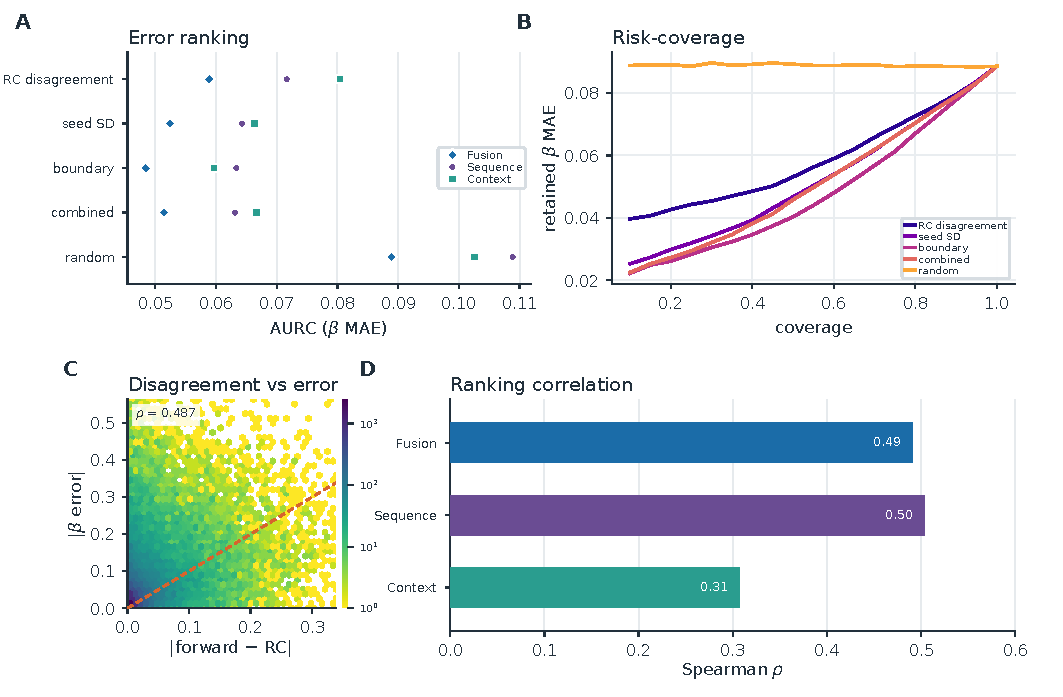
\includegraphics[width=\textwidth]{fig6_uncertainty.pdf}
\caption{\textbf{Forward/reverse-complement disagreement helps identify less reliable predictions.}
\textbf{a}, Area under the error-versus-retained-fraction curve (AURC) for each uncertainty score at seed 42; lower values indicate better error ranking.
\textbf{b}, Fusion $\beta$ MAE as less reliable predictions are removed, compared with random removal.
\textbf{c}, Disagreement versus absolute $\beta$ error for 26,570 held-out CpGs. Colour shows counts on a log scale; the dashed line marks equal values of the two measures.
\textbf{d}, Spearman correlation between disagreement and prediction error, averaged across seeds 42--44. Per-seed results and confidence intervals from resampling 1-Mb blocks are in Source Data. These scores rank reliability but do not provide validated prediction intervals.}
\label{fig:uncertainty}
\end{figure}

\begin{figure}[H]
\centering
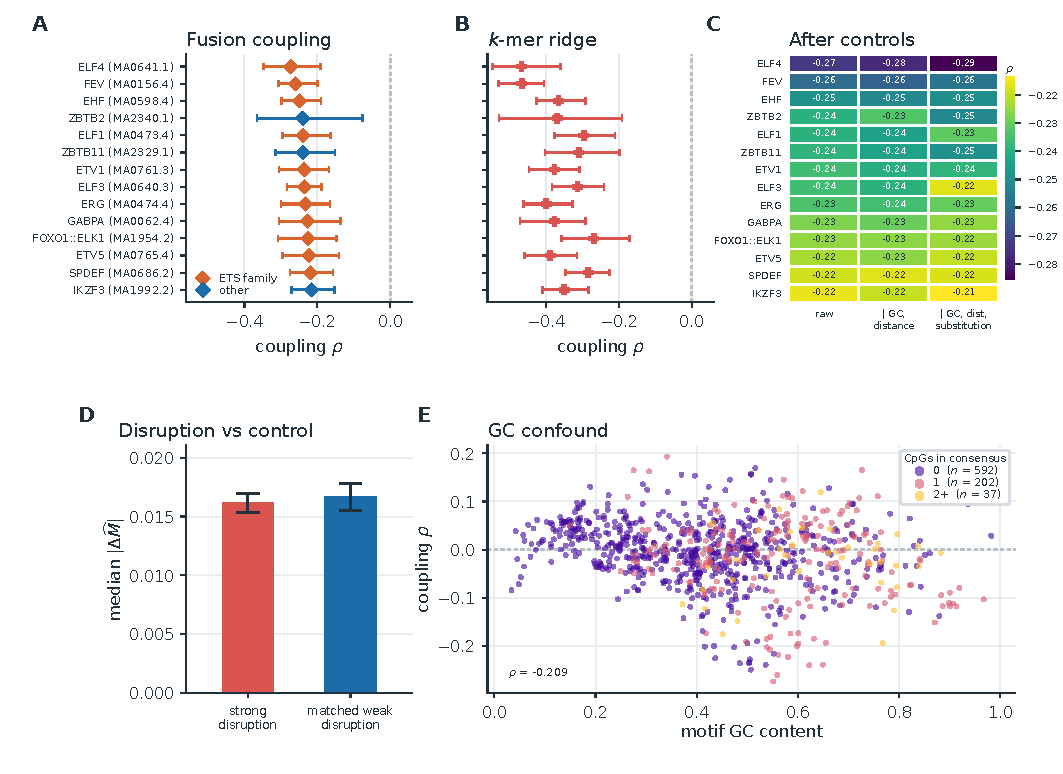
\includegraphics[width=\textwidth]{fig7_motif_controls.pdf}
\caption{\textbf{Motif patterns do not establish learned transcription factor binding.}
\textbf{a}, The 14 JASPAR CORE vertebrate motifs with the strongest correlations between motif disruption and fusion-predicted $\Delta\widehat{M}$. Orange marks related ETS motifs sharing the GGAA core.
\textbf{b}, Correlations for the same motifs using the $k$-mer ridge model.
\textbf{c}, Correlations before and after controlling for GC content, variant--CpG distance and base-change type.
\textbf{d}, Median $|\Delta\widehat{M}|$ for 11,525 variants with strong motif disruption and 9,881 matched controls with weak disruption. Intervals in \textbf{a}, \textbf{b} and \textbf{d} use resampling of 1-Mb blocks.
\textbf{e}, Correlation with predicted effects versus motif GC content for all 831 motifs, coloured by the number of CpGs in each motif's consensus sequence.}
\label{fig:motifs}
\end{figure}

\end{document}